\documentclass[12pt]{beamer}

\usetheme[progressbar=frametitle]{metropolis}
\usepackage{appendixnumberbeamer}

\usepackage{booktabs}
\usepackage[scale=2]{ccicons}

\usepackage{pgfplots}
\usepgfplotslibrary{dateplot}

\usepackage{xspace}
\newcommand{\themename}{\textbf{\textsc{metropolis}}\xspace}

\usepackage[font={small,it}]{caption}
\usepackage{graphicx,wrapfig,lipsum}

\title{Hilbert Curve}
\subtitle{ERA Praktikum}
\date{\today}
%\date{}
\author{Valentin Kostadinov, Mark Bley}
\institute{Technical University of Munich}
% \titlegraphic{\hfill\includegraphics[height=1.5cm]{logo.pdf}}

\begin{document}

\maketitle

\begin{frame}{Table of contents}
  \setbeamertemplate{section in toc}[sections numbered]
  \tableofcontents[hideallsubsections]
\end{frame}

%TODO
%introduction/motivation
\section{Introduction}

\begin{frame}[fragile]{Introduction}
    \begin{itemize}
        \item space filling curve (fills a square)
        \item store 2D Data in 1D linear order
        \item used in CS image processing
        \item can also be extruded to fill 3D space (cube)
    \end{itemize}
\end{frame}

\section{Visualization}


\begin{frame}[fragile]{Visualization}
%------------------------------------------
    \begin{center}
        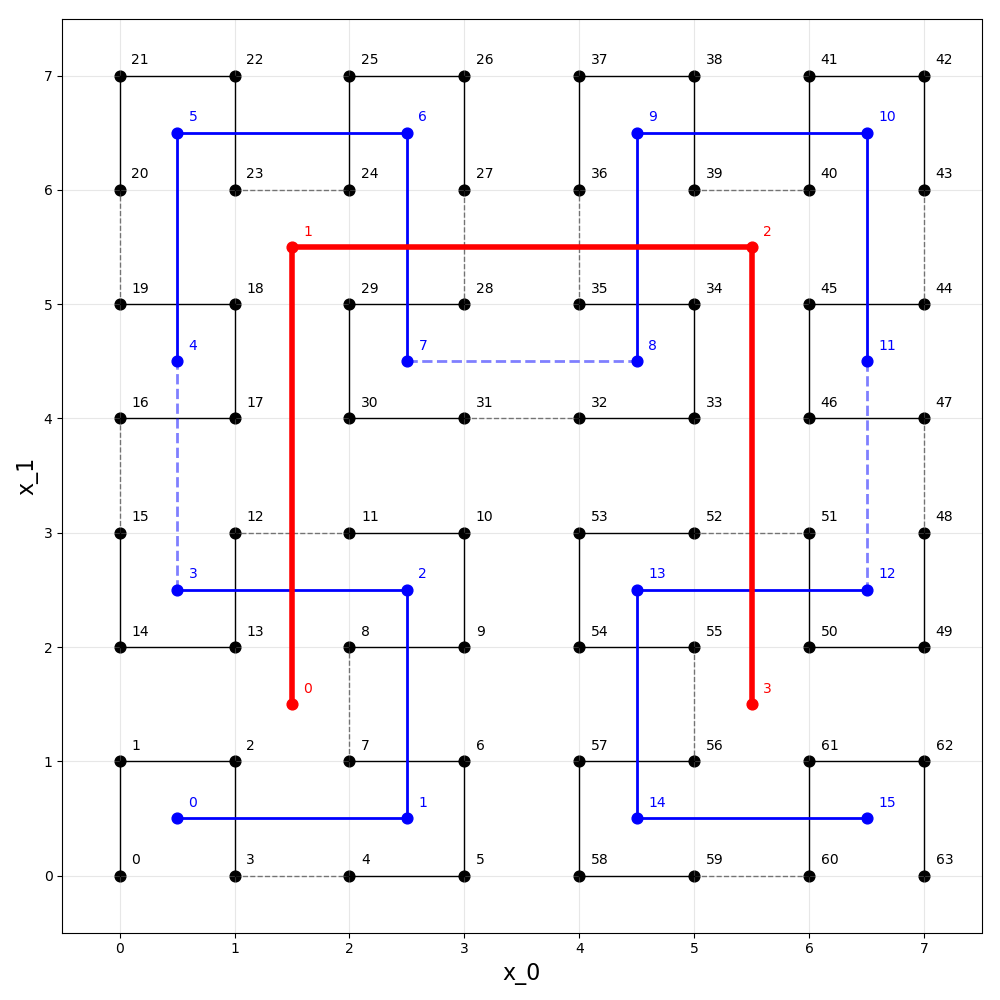
\includegraphics[width=\textwidth,height=0.8\textheight,keepaspectratio]
        {../img/hilbert-sample.png}
    \end{center}
\end{frame}



\section{Demo}

\end{document}
